% What key issues in ocean physics do we want to try to understand, what measurements to make and how.
\subsection{Scientific Motivation}
% Introduction / Motivation

Coastal ocean areas -– the marine areas that extend from the coastline
to the continental slope, comprising the totality of the continental
shelf -– constitute extremely dynamic regions that are forced by a
large variety of agents. They are characterized by complex topography
and coastline boundary and host a broad set of processes operating at
diverse spatial and temporal scales. They are among the most
productive and commercially important regions of the ocean, benefiting
from the combination of terrestrial inputs of organic and inorganic
material from river discharges and the renewal of nutrients from the
upwelling of deep water. Not surprisingly coastal ocean areas
accommodate the vast majority of human activities related to the sea,
including major economic activities such as fisheries, offshore
aquaculture and wind energy.
 
The coastal ocean shapes the two-way interaction between the deep
ocean/ocean basins and the coastal populations and human
societies. They determine, for example, how extreme events or
responses to low period and global changes are transmitted from the
deep ocean to coastal populations, and how anthropogenic influences
originating from the continents are redistributed, while impacting the
maritime environment. This explains why these regions are more
directly affected by anthropogenic pressures.
 
% To understand and ultimately predict the evolution of the different
% processes that take place in the coastal ocean, is of vital importance
% to protect human life at sea and on the coast, to support the blue
% economy and to manage and preserve this rich marine environment.

This environment also plays a significant role in security and defence
needs of all nations. This importance becomes particularly evident to
policy makers and public opinion during significant events such as
those that affected the Portuguese coast during the last two
decades. In the Entre-os-Rios tragedy (March 2001)
\footnote{\url{https://en.wikipedia.org/wiki/Hintze_Ribeiro_disaster}},
caused by the collapse of the Hintze Ribeiro bridge across the Douro
River located more than 30 km inland from the coastline, the
combination of strong river discharge and strong shelf circulation
promoted by downwelling winds led to an astonishing rapid transport of
victims' bodies along the coast, covering more than a thousand
kilometers to reach the northern Spanish and the French coastlines.

During the \emph{Prestige} oil
spill\footnote{\url{https://en.wikipedia.org/wiki/Prestige_oil_spill}},
in November-December 2002, the slope % intensified flow that develops
% along the continental slopes of Western Portugal-Northern Spain
distributed the oil spill that resulted from the breaking and sinking
of the tanker which extended for over one thousand kilometers of the
coastlines of Spain, Portugal and France, transforming a local problem
into a European-wide crisis. More recently the conditions over the
coastal ocean domain determined the final evolution of Hurricane
Leslie (13-14 October 2018) and the impacts on the Portuguese
mainland.
 
Central to the capacity to provide effective support during these
major accidents at sea was the ability to describe and forecast the
evolution of coastal ocean conditions observed offshore, in particular
to track the rapid adjustment in response to changing forcing and to
correctly incorporate/describe the importance of subsurface processes
such as the slope current.
 
These events highlight:

\begin{itemize}[noitemsep,topsep=0pt,parsep=0pt,partopsep=0pt]
  
\item the importance of assimilation models that are fed with actual
  observations to provide forecasts consistent with the evolution of
  coastal ocean conditions

\item the rapid adjustment of coastal ocean conditions to changes in
  forcing agents leading to significant changes of conditions after
  one or two days

\item The crucial role of subsurface conditions and processes
 
\end{itemize}

In these events, as well as in many routine activities such as support
for Search And Rescue operations, to Blue Economy sectors or Rapid
Environmental Assessment for naval operations, the capacity to observe
the actual conditions that affect the water column over the coastal
ocean regions of interest in such a way that these observations can
effectively feed the operational models with assimilation, play a
critical role. This remains a challenge not only due to the large
diversity of processes operating at many different spatial and
temporal scales in the coastal ocean but also due to the concentration
of human activities which can dramatically constraint or render
unviable, monitoring activities.

Not surprisingly these constraints translate to serious limitations in
the use of assimilation in operational forecasting of coastal ocean
areas. In the European landscape, for example, a recent survey
promoted among members of \texttt{EuroGOOS} and its related network of
Regional Operational Oceanographic Systems \cite{capet2020} showed the
limited use of data assimilation in European forecast
centers. Assimilation is largely restricted to physical variables and,
among these, to surface observations collected by satellites and water
column data collected by \texttt{ARGOS} profiles and, to a lesser
extent to observations collected during regular programs (fixed
platforms, cruises, glider lines). Assimilation of surface currents,
for example collected by HF radar systems, is still very limited. The
same study also highlighted the limited use of biogeochemical models
(BGC) and variables.
 
Existing operational forecast systems are frequently based on a number
of assumptions that greatly limit the capacity of these models to
describe the actual conditions observed in a given coastal ocean
domain of interest at a given window of time. For example, many of
these models incorporate the influence of freshwater discharges in the
coastal ocean environment in the form of climatological monthly mean
values associated with major rivers \cite{marta012}.  In operational
support scenarios, these models can substantially diverge from
real-world conditions which can be dictated by discharges from major
rivers that substantially differ from the climatological picture or by
large influence of small rivers and fresh water sources which are not
included in the forecast models.
 
These challenges are even more daunting in BGC models, especially
those used in operationally. Components of these models are typically
defined in terms of variable dependencies and parameters that are
derived from climatology or based on a limited set of past
observations. Assimilation in BGC models is largely restricted to the
use of surface distributions of chlorophyll provided by satellite
observations combined by established dependencies to infer other
variable distributions. As a consequence the picture described by
these models is frequently far from conditions actually observed and
the capacity to respond to operational requests remains limited (see
for example Figs. 5 and 6 from \cite{marta012}).
 
% Improving the capacity for operational models to simulate and forecast
% the real conditions prevailing in a given geographical domain can
% translate to a significant impact in many different areas related to
% the coastal ocean environment. For example
Improving the ability of a BGC model to characterize and forecast the
phyto- and zoo-plankton distributions in the water column is not only
key to understanding the main processes shaping the coastal ocean
ecosystems but essential to consistently forecast the development of
algal blooms impacting coastal fisheries or to improve the capacities
of underwater visibility models to support diver operations and beach
access to the public.
 
\begin{quote}
  \textsf{General Objective 1:} \proj will explore and evaluate
  strategies to build the initialization and assimilation fields to be
  used by BGC models applied to a coastal ocean area. The approach
  would be similar to the overall strategy used in the context of
  Rapid Environmental Assessment for Navy operations and will leverage
  observations from autonomous vehicles, traditional methods such as
  ship-based measurements and opportunistic measurements using low
  cost sensors, exploring synergies between dedicated surveys and
  opportunistic observations.
\end{quote}
 
By improving the capacity to observe and forecast a coastal ocean
domain of interest the approach followed by \proj will also
significantly contribute to improving our understanding of how the
combination of physical and biogeochemical processes may impact the
coastal ocean. Critical impact can occur in those areas where the
prevailing physical processes can promote a rapid intake of nutrients
into the upper layers that boost rapid development at all levels of
the trophic chain. In the coastal ocean environment those important
vertical motions linking the surface conditions with the subsurface
processes can be promoted by the presence of the coastal boundary, by
the complex topography of the continental shelf and slope or by the
vertical mixing that occurs at different scales (e.g cold water
cascade events at regional scale, vertical mixing associated with
solitons at submesoscale). They are particularly expressive in the
areas of the coastal ocean cut by narrow submarine canyons. These deep
incisions of the continental slope extending over the shelf are a
ubiquitous features of coastal ocean areas.  They interact with the
wind driven shelf circulation promoting for example, a rapid and
intensified response to upwelling favorable winds \cite{she00} which,
in the case of a long submarine canyon, can be sustained in time
despite the variability, leading to a persistent upwelling condition
\cite{allen00}.

\begin{quote} 
  \textsf{General Objective 2:} \proj will articulate a broad range of
  observation systems in combination with data assimilation models to
  acquire unprecedented insight on the integrated physical and
  biogeochemical processes that are associated with these particularly
  important areas of the coastal ocean environment.
\end{quote} 

\subsection{The domain: \naze, Portugal}
\label{sec:naz}

\begin{figure}[!b]
  \vspace{-0.5cm} 
  \centering 
  \subfigure[Map of Portugal and the study area highlighted with the red
  rectangle.]{\label{fig:po-map}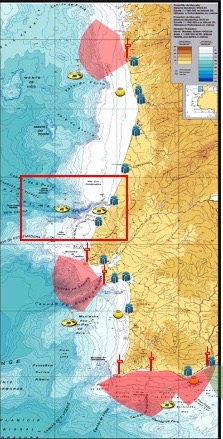
\includegraphics[scale=0.5]{fig/po-map.jpeg}}
  \hspace{+0.3cm} 
  \subfigure[Zoomed in bathymetry showing the \naz canyon-Berlengas
  area (isobaths with depth in meters) and its environment including
  the placement of the two buoys.]{\label{fig:domain}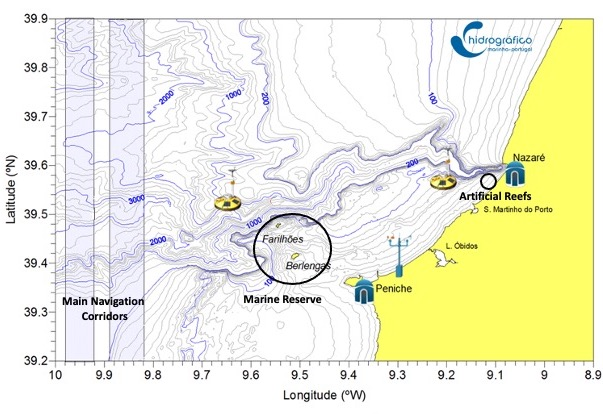
\includegraphics[scale=0.55]{fig/domain.jpg}}
  \caption{\subref{fig:po-map} \& \subref{fig:domain} show detailed
    views of the proposed study area for \proj off the coast of
    mainland Portugal. The \naz Canyon is a significant feature of
    this area and a driver for the bio-geophysics of the domain. The
    shaded blue area is the expected glider operations region which
    will inform the model about boundary conditions and off-shore
    waters being entrained into the canyon.}
  \label{fig:studyarea-1}
\end{figure}

\proj will focus on the area of influence of \naz Canyon located in
the central part of the western Portuguese coast and broadly extending
from 39.2$^{\circ}$N (south of Peniche) to 39.9$^{\circ}$N north of
\naz (Fig. \ref{fig:po-map}). This is a coastal ocean area well
exposed to the influence of the North Atlantic and marked by
important topographic features such as:

\begin{itemize}[noitemsep,topsep=0pt,parsep=0pt,partopsep=0pt]

\item important changes of the continental margin associated with the
  transition from the large Estremadura Plateau to the south, to the
  relatively narrow shelf north of \naz

\item the presence of a long and narrow submarine canyon – the \naz
  canyon that extends for more than 200 km from the head, just a few
  hundreds of meters from the beach of \naze, incising the shelf into
  abyssal areas

\item the presence of island environments -– the Berlengas archipelago
  located a few tens of kilometers offshore the coast which is a
  \texttt{Natura2000} site recognized as a unique repository of
  species and habitat diversity on the western boundary of Europe. It
  was recently classified by UNESCO as a Biosphere Reserve. The
  biogeographic, geologic and oceanographic settings of this region,
  accentuated by the presence of the \naz canyon, are crucial for high
  levels of biological productivity and biodiversity, that induce
  dynamic ecological processes and support many ecosystem services

\end{itemize}

% The region offers one of the longest and
% deepest canyon's in continental Europe with powerful tidal pumping,
% generation of internal waves, seasonal wind forcing promoting canyon
% driven upwelling and large upwelling filaments extending offshore for
% hundreds of kilometers from shore with dispersal along the south and
% the northern coasts as well as into the Atlantic.  Thus this region is
% very dynamic with frequent and rapid changes in water column
% properties, making it ideal for testing our model and sampling skills.
% The long canyon and the presence of two islands just offshore provide
% an interesting range of bio-geophysical phenomenon not observed
% elsewhere including routine 30 meter waves in the surf zone; as a
% result \naz is renowned as a surfing location
% ~\footnote{\url{https://www.youtube.com/watch?v=GJc4Ir78KdE}, and
%   \url{https://www.youtube.com/watch?v=74pnrYPozcU}} with substantial
% media coverage especially in the English speaking world.  Equally, the
% Portuguese Hydrographic Institute (Instituto Hidrogr\'{a}fico or
% \inste)~\footnote{\url{https://www.hidrografico.pt/}} maintains two
% real-time multi-parameter buoys as well as tide gauges in the vicinity
% of the canyon. We propose to leverage \inste's twice yearly
% maintenance visits by their research vessels to augment our logistical
% support and therefore propose to hold the experiment at one of those
% times.

% This is a coastal ocean area well exposed to the influence of the
% North Atlantic and marked by important topographic features. These
% include the important changes of the continental margin associated
% with the transition from the large Estremadura Plateau in the south,
% to the relatively narrow shelf north of \naze. In addition, this
% includes the presence of a long and narrow submarine \naz Canyon, that
% extends for more than 200 kms from the head, just a few hundreds of
% meters from the beach of \naze, incising the shelf into abyssal areas,
% the presence of island environments -– the Berlengas Archipelago,
% located a few tens of kilometers offshore\footnote{This is a
%   Natura2000 site recognized as a unique repository of genetic species
%   and habitat diversity on the western boundary of Europe and was
%   recently classified by UNESCO as Biosphere Reserve}. The
% biogeographic, geologic and oceanographic settings of this region,
% accentuated by the presence of the \naz Canyon, are crucial for high
% levels of biological productivity and biodiversity and induce dynamic
% ecological processes and support many ecosystem services
% \cite{tyler09,cunha11}.  

The \naz Canyon area of influence is not directly impacted by major
riverine outflows. The main rivers influencing the western Portuguese
continental margin are the Douro (located about 170 km to the north of
\naze) and the Tagus (located at about 100 km to the south) with
smaller contributions from the Mondego (50 km to the north). During
the winter and early spring the combined influence of the Douro and
other smaller rivers such as the Mondego reach the \naz Canyon area
during periods of northerly winds and upwelling conditions, appearing
as a low salinity water plume occupying the first 30 m of the water
column and extending over the complete shelf as the result of offshore
transport associated with the prevailing upwelling conditions. The
influence of the Tagus River on the area is less clear, largely due to
the combination of the large Estremadura Plateau with the shallow
ridge between Cape Carvoeiro and Berlengas areas and associated
circulation characteristics. More expressive for the conditions in the
area is the contribution of the small riverine sources that indent the
\naze-Peniche coast during periods of important precipitation. These
include the contributions of the small Alcoa and Tornadas rivers, of a
large number of very small fresh water courses (ribeiras) or from the
Obidos Lagoon. Previous observations have showed \cite{martins10} that
these contributions combine fresh waters with high turbidity and high
nutrient content that can extend its influence over the complete
shelf.

The evolution of wind forcing and wave conditions affecting this area
is largely determined by the seasonal migration of the Azores High
Pressure System. From May to September the Azores High is typically
located at its northernmost position, offshore the Iberian
Peninsula. During this period, the western Portuguese margin is
located on the eastern branch of the High, under the influence of
persistent (upwelling favorable) northerly winds that during the
summer months, are reinforced by the establishment of a thermal low
over central Iberia. The area is also protected from the influence of
synoptic low pressure systems, showing typically low energy swells
(although affected by locally generated sea breeze
circulation). During the winter months the conditions prevailing along
the western Portuguese margin are largely associated with the phase of
the winter North Atlantic Oscillation (NAO). During the negative phase
of the winter NAO the Azores High is typically located southwest of
the Iberian Peninsula and the western Portuguese coast is under the
influence of westerly and southwesterly wind forcing that frequently
promote downwelling conditions. During those periods the area is also
exposed to the direct influence of synoptic low pressure systems and
associated highly energetic waves. During the positive phases of the
winter NAO, the Azores High remains at northward latitudes leading to
frequent periods of northerly winds and upwelling conditions along the
western Portuguese margin. During these periods the area is largely
protected from the direct influence of low pressure synoptic systems
and shows a less energetic wave regime in general, although impacted
by large swells that are generated far in the North Atlantic.

The atmospheric forcing conditions described above establish some
complex dynamics in the \naz canyon area of influence, marked by the
interactions of the shelf and slope circulation with the canyon
topography and island environments and by the manifestation of
important meso-scale features such as the upwelling filament of Cape
Carvoeiro. In addition, the rich topography of the area also promotes
complex tidal dynamics. Barotropic tidal currents along the western
Portuguese margin are in general dominated by the semidiurnal lunar
constituent (M2), within a period of 12 hours and 25 minutes.  In the
shelf north of \naz canyon the barotropic tidal current magnitudes are
dominated by the M2 constituent and show magnitudes of 5-10 cm/s. To
the south of Peniche, the large and shallow Estremadura Plateau
constitutes an area of intensification of the barotropic tidal
currents, both for the dominant constituent (M2) that shows magnitudes
of order 10 cm/s, as well as for the diurnal constituents such as the
lunar diurnal constituent (K1) that shows magnitudes comparable with
M2 \cite{marta06,quaresma13}. A particular area of interest, is the
shallow ridge located between Cape Carvoeiro and Berlengas Islands
where total currents can on some occasion, reach 50-60 cm/s.


The interaction of the barotropic tide with the shelf edge topography
in the presence of stratification opens the potential for generation
of internal tidal motions that propagate offshore to the deep ocean
domain and, if the stratification conditions of the continental shelf
allow, also onshore. The effect of these internal motions generated at
the shelf edge however remains largely confined to the outer and
mid-shelf, the waves being dissipated before reaching the inner shelf
environment. By cutting the complete continental shelf, the \naz
canyon opens the possibility for internal tidal motions to be
generated at positions along the canyon rim located very close to the
shore, impacting the mid and inner shelf environments if
stratification conditions allow the onshore propagation of these
waves. An example of those impacts was presented by \cite{quaresma07}
based on observations of solitons generated at the canyon rim and
propagating towards the inner continental shelf impacting the bottom
sedimentary cover and promoting vertical mixing.


% The seasonal evolution of wind forcing and wave conditions that affect
% this area are largely determined by evolution of the Azores High
% Pressure System. From May to September the Azores High is typically
% located at northern positions, offshore the Iberian Peninsula. The
% western Portuguese margin is then located on the eastern branch of the
% High, under the influence of persistent (upwelling favorable)
% northerly winds that during the summer months are reinforced by the
% establishment of a thermal low over central Iberia. The area is also
% protected from the influence of synoptic low pressure systems, showing
% typically low energy swells (although affected by locally generated
% seas associated with the sea breeze circulation). During winter months
% the conditions prevailing along the western Portuguese margin are
% largely associated with the phase of the winter North Atlantic
% Oscillation (NAO). During the negative phase of the winter NAO the
% Azores High is typically located south of the Iberian Peninsula and
% the western Portuguese coast is under the influence of westerly and
% southwesterly wind forcing that frequently promote downwelling
% conditions and is exposed to the influence of synoptic low pressure
% systems and an highly energetic wave regime. During positive phases of
% the winter NAO the Azores High remains at a high latitude leading to
% frequent periods of northerly winds and upwelling conditions. During
% those periods the area is largely protected from the influence of
% swells generated in the North Atlantic.
 
% Tidal motions in the area are dominated by the semi-diurnal lunar
% constituent although in the large and shallow Estremadura plateau, in
% the south of the area, tidal currents over the shelf are generally of
% moderate expression \kc{with speeds up to } based on current meters
% moorings and bottom mounted ADCPs.  Much larger tidal motions are
% observed near bottom depths inside the \naz Canyon, as the result
% of bottom focusing of internal tide energy generated at the canyon
% rim. 
 
% The interaction of the barotropic tide with the shelf edge topography
% in the presence of stratification opens the potential for generation
% of internal tidal motions that propagate offshore to the deep ocean
% domain and, if the stratification conditions of the continental shelf
% allow, also onshore. The effect of these internal motions generated at
% the shelf edge however remains, the waves being dissipated before
% reaching the inner shelf environment. The major topography of \naz
% Canyon however, allows that internal tidal motions can be generated in
% positions along the canyon rim very close to the
% shore. \cite{quaresma07} % Quaresma etal.
% for example showed the expression and impact of solitons that
% propagate towards the inner continental shelf impacting the nutrient
% fluxes to the photic layer and the near bottom sedimentary cover.

